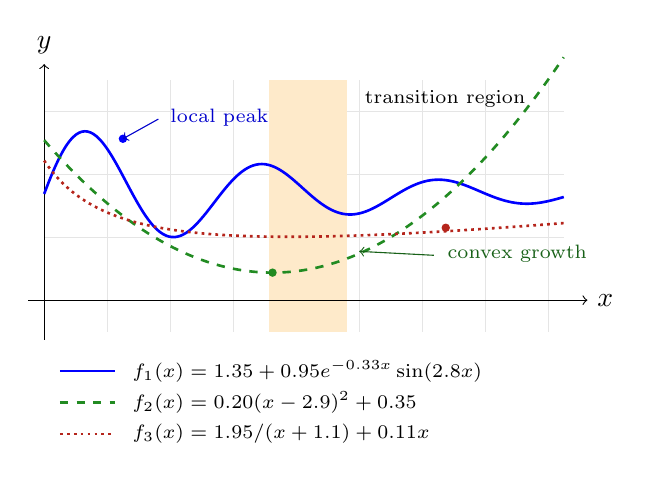
\begin{tikzpicture}[scale=1.0]
  \draw[gray!20, step=0.8] (0.0,-0.4) grid (6.6,2.8);
  \fill[YellowOrange!18] (2.85,-0.4) rectangle (3.85,2.8);

  \draw[->] (-0.2,0.0) -- (6.9,0.0) node[right] {\(x\)};
  \draw[->] (0.0,-0.5) -- (0.0,3.0) node[above] {\(y\)};

  \draw[line width=0.95pt, Blue, domain=0.0:6.6, samples=180, smooth]
    plot (\x, {1.35 + 0.95*exp(-0.33*\x)*sin(2.8*\x r)});
  \draw[line width=0.95pt, ForestGreen, dashed, domain=0.0:6.6, samples=150, smooth]
    plot (\x, {0.20*(\x-2.9)^2 + 0.35});
  \draw[line width=0.95pt, BrickRed, dash pattern=on 1pt off 1.5pt, domain=0.0:6.6, samples=150, smooth]
    plot (\x, {1.95/(\x+1.1) + 0.11*\x});

  \node[font=\scriptsize, anchor=west] at (3.95,2.56) {transition region};

  \filldraw[Blue] (1.0,2.05) circle (1.3pt);
  \filldraw[ForestGreen] (2.9,0.35) circle (1.3pt);
  \filldraw[BrickRed] (5.1,0.92) circle (1.3pt);

  \draw[->, thin, Blue!80!black] (1.45,2.3) -- (1.0,2.05);
  \node[font=\scriptsize, Blue!80!black, anchor=west] at (1.48,2.32) {local peak};

  \draw[->, thin, ForestGreen!70!black] (4.95,0.57) -- (4.0,0.62);
  \node[font=\scriptsize, ForestGreen!70!black, anchor=west] at (5.0,0.59) {convex growth};

  \draw[line width=0.95pt, Blue] (0.2,-0.90) -- (0.9,-0.90);
  \node[font=\scriptsize, anchor=west] at (1.0,-0.90) {\(f_1(x)=1.35+0.95e^{-0.33x}\sin(2.8x)\)};

  \draw[line width=0.95pt, ForestGreen, dashed] (0.2,-1.30) -- (0.9,-1.30);
  \node[font=\scriptsize, anchor=west] at (1.0,-1.30) {\(f_2(x)=0.20(x-2.9)^2+0.35\)};

  \draw[line width=0.95pt, BrickRed, dash pattern=on 1pt off 1.5pt] (0.2,-1.70) -- (0.9,-1.70);
  \node[font=\scriptsize, anchor=west] at (1.0,-1.70) {\(f_3(x)=1.95/(x+1.1)+0.11x\)};
\end{tikzpicture}
